% =============================================================================
%  Diplomado en Data Science Aplicada con Python para la Toma de Decisiones
%  Clase 16: Evaluación Rigurosa de Clasificadores --- Train/Test, ROC y PR
%  Arca Continental Ecuador | UDLA
%
%  Compilar: pdflatex -shell-escape presentacion.tex (x2 para refs)
% =============================================================================
\documentclass[aspectratio=169, 11pt]{beamer}

\usepackage[T1]{fontenc}
\usepackage[utf8]{inputenc}
\usepackage[spanish,es-noshorthands]{babel}
\usepackage{FiraSans}
\usepackage{FiraMono}
\renewcommand{\familydefault}{\sfdefault}
\usepackage{graphicx}
\usepackage{tikz}
\usetikzlibrary{arrows.meta, positioning, shapes.geometric, shapes.misc,
  calc, fit, decorations.pathreplacing, backgrounds}
\usepackage{fontawesome5}
\usepackage{minted}
\usepackage{tcolorbox}
\tcbuselibrary{minted, skins, breakable}
\usepackage{booktabs}
\usepackage{colortbl}
\usepackage{multicol}
\usepackage{hyperref}
\usepackage{calc}
\usepackage{amsmath}

\definecolor{arcaRed}{HTML}{C82B40}
\definecolor{arcaDark}{HTML}{6B1525}
\definecolor{udlaCrimson}{HTML}{A31545}
\definecolor{arcaGray}{HTML}{F5F5F5}
\definecolor{arcaLightGray}{HTML}{EBEBEB}
\definecolor{textDark}{HTML}{2D2D2D}
\definecolor{textMuted}{HTML}{6B7280}
\definecolor{codeGreen}{HTML}{16A34A}
\definecolor{codeBlue}{HTML}{2563EB}
\definecolor{codeOrange}{HTML}{EA580C}
\definecolor{codePurple}{HTML}{7C3AED}

\usetheme{default}
\usecolortheme{default}
\setbeamertemplate{navigation symbols}{}
\setbeamertemplate{footline}{}
\setbeamertemplate{headline}{}
\setbeamercolor{normal text}{fg=textDark}
\setbeamercolor{frametitle}{fg=arcaRed, bg=white}
\setbeamercolor{title}{fg=white}
\setbeamercolor{subtitle}{fg=white!85}
\setbeamercolor{author}{fg=white!80}
\setbeamercolor{date}{fg=white!70}
\setbeamercolor{item}{fg=arcaRed}
\setbeamercolor{subitem}{fg=arcaDark}
\setbeamercolor{block title}{fg=white, bg=arcaRed}
\setbeamercolor{block body}{fg=textDark, bg=arcaGray}
\setbeamercolor{block title alerted}{fg=white, bg=codeOrange}
\setbeamercolor{block body alerted}{fg=textDark, bg=arcaGray}
\setbeamercolor{block title example}{fg=white, bg=codeGreen}
\setbeamercolor{block body example}{fg=textDark, bg=arcaGray}
\setbeamercolor{section in toc}{fg=arcaDark}
\setbeamerfont{frametitle}{size=\Large, series=\bfseries}
\setbeamerfont{title}{size=\huge, series=\bfseries}
\setbeamerfont{subtitle}{size=\large}
\setbeamerfont{author}{size=\normalsize}
\setbeamerfont{date}{size=\small}
\setbeamerfont{block title}{size=\normalsize, series=\bfseries}
\setbeamerfont{footnote}{size=\tiny}
\setbeamertemplate{itemize item}{\scriptsize\raise1.5pt\hbox{\color{arcaRed}$\blacktriangleright$}}
\setbeamertemplate{itemize subitem}{\scriptsize\raise1pt\hbox{\color{arcaDark}$\bullet$}}
\setbeamertemplate{enumerate items}[default]
\setbeamercolor{enumerate item}{fg=arcaRed}

\setbeamertemplate{headline}{%
  \begin{tikzpicture}[remember picture, overlay]
    \fill[arcaDark] (current page.north west) rectangle
      ([yshift=-0.7cm]current page.north east);
    \node[anchor=west, inner sep=0pt] at
      ([xshift=0.6cm, yshift=-0.35cm]current page.north west)
      {
\includegraphics[height=0.45cm]{../logo_udla_white.png}};
    \node[anchor=east, inner sep=0pt] at
      ([xshift=-0.6cm, yshift=-0.35cm]current page.north east)
      {
\includegraphics[height=0.45cm]{../ArcaContinental_white.png}};
  \end{tikzpicture}%
  \vspace{0.7cm}%
}

\setbeamertemplate{footline}{%
  \begin{tikzpicture}[remember picture, overlay]
    \node[anchor=south east, font=\scriptsize\bfseries\color{arcaRed}] at
      ([xshift=-0.5cm, yshift=0.15cm]current page.south east)
      {\insertframenumber};
  \end{tikzpicture}%
  \vspace{0.3cm}%
}

\setbeamertemplate{frametitle}{%
  \vspace{0.25cm}%
  \usebeamerfont{frametitle}\usebeamercolor[fg]{frametitle}\insertframetitle%
  \par\vspace{2pt}%
  \begin{tikzpicture}
    \fill[arcaRed] (0,0) rectangle (3cm, 1.5pt);
    \fill[arcaLightGray] (3cm,0) rectangle (\textwidth, 0.5pt);
  \end{tikzpicture}%
  \vspace{0.1cm}%
}

\newtcblisting{pyblock}[1][]{%
  listing engine=minted, minted language=python, minted style=friendly,
  minted options={fontsize=\small, linenos=false, breaklines=true, python3=true},
  colback=arcaGray, colframe=arcaRed, left=4pt, right=4pt, top=4pt, bottom=4pt,
  boxrule=0pt, leftrule=3pt, arc=2pt, listing only, #1}

\newtcblisting{outputblock}[1][]{%
  listing engine=minted, minted language=text, minted style=bw,
  minted options={fontsize=\small, breaklines=true},
  colback=white, colframe=arcaLightGray, left=4pt, right=4pt, top=4pt, bottom=4pt,
  boxrule=0.5pt, arc=2pt, listing only,
  title={\small\faTerminal\hspace{6pt}Output}, coltitle=textMuted,
  fonttitle=\small\ttfamily, colbacktitle=white, #1}

\newcommand{\sectionframe}[2]{%
  \begingroup
  \setbeamertemplate{headline}{}%
  \setbeamertemplate{footline}{}%
  \begin{frame}[plain, noframenumbering]
    \begin{tikzpicture}[remember picture, overlay]
      \fill[arcaRed] (current page.south west) rectangle (current page.north east);
      \node[anchor=center, text=white, font=\Huge\bfseries, text width=12cm,
            align=center] at ([yshift=0.5cm]current page.center) {#1};
      \node[anchor=center, text=white!80, font=\large, text width=10cm,
            align=center] at ([yshift=-0.8cm]current page.center) {#2};
    \end{tikzpicture}
  \end{frame}
  \endgroup
}

\title{Diplomado en Data Science Aplicada\\con Python para la Toma de Decisiones}
\subtitle{Clase 16: Evaluación Rigurosa --- Plotly, Train/Test, ROC y PR}
\author{Carlos Enrique Mosquera Trujillo}
\date{15 de Abril, 2026}

\begin{document}

% ── PORTADA ──────────────────────────────────────────────────────────────────
{
\setbeamertemplate{headline}{}
\setbeamertemplate{footline}{}
\begin{frame}[plain, noframenumbering]
  \begin{tikzpicture}[remember picture, overlay]
    \fill[arcaDark] (current page.south west) rectangle (current page.north east);
    \fill[arcaRed] ([yshift=-3.5cm]current page.north west) rectangle
      ([yshift=-4.2cm]current page.north east);
    \node[anchor=west, inner sep=0pt] at
      ([xshift=1cm, yshift=-1.5cm]current page.north west)
      {
\includegraphics[height=1cm]{../logo_udla_white.png}};
    \node[anchor=east, inner sep=0pt] at
      ([xshift=-1cm, yshift=-1.5cm]current page.north east)
      {
\includegraphics[height=1cm]{../ArcaContinental_white.png}};
  \end{tikzpicture}
  \vspace{2.5cm}
  \begin{center}
    {\usebeamerfont{title}\usebeamercolor[fg]{title}\inserttitle\par}
    \vspace{0.4cm}
    {\usebeamerfont{subtitle}\usebeamercolor[fg]{subtitle}\insertsubtitle\par}
    \vspace{0.6cm}
    {\usebeamerfont{author}\usebeamercolor[fg]{author}\insertauthor\par}
    \vspace{0.15cm}
    {\usebeamerfont{date}\usebeamercolor[fg]{date}\insertdate\par}
  \end{center}
\end{frame}
}

% ── MÓDULO 4 ─────────────────────────────────────────────────────────────────
{
\setbeamertemplate{headline}{}
\setbeamertemplate{footline}{}
\begin{frame}[plain, noframenumbering]
  \begin{tikzpicture}[remember picture, overlay]
    \fill[arcaDark] (current page.south west) rectangle (current page.north east);
    \node[anchor=center, text=white, font=\Large\bfseries, text width=12cm,
          align=center] at ([yshift=1cm]current page.center)
      {Módulo 4 --- clase 3};
    \node[anchor=center, text=white!90, font=\huge\bfseries, text width=12cm,
          align=center] at ([yshift=-0.3cm]current page.center)
      {Machine Learning Supervisado};
  \end{tikzpicture}
\end{frame}
}

% ── ROADMAP ─────────────────────────────────────────────────────────────────
\begin{frame}[shrink=22]{Hoja de Ruta de Hoy}
  \vspace{-4pt}
  \begin{center}
  \begin{tikzpicture}[
    node distance=0.35cm,
    roadstep/.style={rectangle, rounded corners=4pt, draw=arcaRed, fill=arcaRed!8,
                 minimum width=11cm, minimum height=0.65cm,
                 font=\footnotesize\bfseries\color{arcaDark}, align=left,
                 text width=10cm, inner sep=6pt},
    num/.style={circle, fill=arcaRed, text=white, font=\scriptsize\bfseries,
                minimum size=0.5cm, inner sep=0pt},
  ]
    \node[roadstep] (s0) {\hspace{0.8cm}El mapa de ML: supervisado, no supervisado, tareas};
    \node[roadstep, below=of s0] (s1) {\hspace{0.8cm}Plotly: la tercera librería --- interactiva};
    \node[roadstep, below=of s1] (s2) {\hspace{0.8cm}Nuevo dataset: predicción de ACV (stroke)};
    \node[roadstep, below=of s2] (s3) {\hspace{0.8cm}Train/Test Split --- evaluar de verdad};
    \node[roadstep, below=of s3] (s4) {\hspace{0.8cm}Curva ROC y AUC};
    \node[roadstep, below=of s4] (s5) {\hspace{0.8cm}Curva Precision-Recall (la correcta para desbalanceados)};
    \node[roadstep, below=of s5] (s6) {\hspace{0.8cm}Umbral óptimo con lógica de negocio};

    \node[num] at ([xshift=0.45cm]s0.west) {0};
    \node[num] at ([xshift=0.45cm]s1.west) {1};
    \node[num] at ([xshift=0.45cm]s2.west) {2};
    \node[num] at ([xshift=0.45cm]s3.west) {3};
    \node[num] at ([xshift=0.45cm]s4.west) {4};
    \node[num] at ([xshift=0.45cm]s5.west) {5};
    \node[num] at ([xshift=0.45cm]s6.west) {6};
  \end{tikzpicture}
  \end{center}
\end{frame}

% =============================================================================
%  BLOQUE 0: MAPA DE MACHINE LEARNING
% =============================================================================
\sectionframe{El Mapa de Machine Learning}{Para entender dónde estamos parados}

\begin{frame}{Tipos de Aprendizaje}
  \vspace{-4pt}
  {\footnotesize\color{arcaDark}\bfseries
    La pregunta no es \textit{qué modelo usar}, sino \textbf{cómo
    aprende} el modelo. Hay varios paradigmas.}

  \vspace{6pt}
  {\footnotesize
  \begin{tabular}{@{}p{3cm}p{5cm}p{4.5cm}@{}}
    \toprule
    \textbf{Paradigma} & \textbf{Cómo aprende} & \textbf{Ejemplo cotidiano} \\
    \midrule
    \textbf{\color{codeBlue}Supervisado} &
      Le muestro muchos ejemplos \textbf{con la respuesta}. Aprende a mapear $X \to y$. &
      Profesor marca 100 exámenes con la corrección. \\
    \textbf{\color{codePurple}No supervisado} &
      Le doy datos \textbf{sin respuesta}. Encuentra estructura por sí solo. &
      Organizar fotos en álbumes sin decirle categorías. \\
    \textbf{\color{codeGreen}Por refuerzo} &
      Aprende \textbf{probando} en un entorno y recibiendo recompensas. &
      Perro aprende trucos con premios. \\
    \bottomrule
  \end{tabular}
  }

  \vspace{6pt}
  {\footnotesize\color{textMuted}
    \faLightbulb\hspace{4pt} En clases 13--15 ya trabajamos aprendizaje
    \textbf{supervisado} sin nombrarlo. Hoy le ponemos nombre.}
\end{frame}

\begin{frame}{Las Dos Grandes Familias}
  \vspace{-4pt}
  \begin{center}
  \begin{tikzpicture}[
    box/.style={rectangle, rounded corners=4pt, draw=arcaRed, thick,
                minimum width=5.5cm, minimum height=1.6cm,
                font=\footnotesize, align=left, text width=5cm, inner sep=6pt},
  ]
    \node[font=\large\bfseries\color{arcaDark}] (root) at (0, 4) {Machine Learning};

    \node[box, fill=codeBlue!10, draw=codeBlue] (sup) at (-4, 2) {%
      {\bfseries\color{codeBlue}\faTag\ Supervisado}\\[3pt]
      Tenemos \textbf{respuestas correctas} (target $y$).\\
      El modelo aprende la relación $X \to y$.};

    \node[box, fill=codePurple!10, draw=codePurple] (unsup) at (4, 2) {%
      {\bfseries\color{codePurple}\faQuestionCircle\ No Supervisado}\\[3pt]
      \textbf{No hay target}. Solo features $X$.\\
      El modelo descubre estructura oculta.};

    \draw[->, thick, arcaRed] (root) -- (sup);
    \draw[->, thick, arcaRed] (root) -- (unsup);
  \end{tikzpicture}
  \end{center}

  \vspace{8pt}
  {\scriptsize\color{textMuted}
  \begin{itemize}\setlength{\itemsep}{3pt}
    \item[{\color{codeBlue}\scriptsize\faArrowRight}]
      \textbf{Supervisado}: ``aquí están 1000 pacientes con su diagnóstico
      --- predice el próximo''.
    \item[{\color{codePurple}\scriptsize\faArrowRight}]
      \textbf{No supervisado}: ``aquí están 1000 clientes --- agrúpalos
      en segmentos parecidos''.
  \end{itemize}
  }
\end{frame}

\begin{frame}{Supervisado: Regresión vs Clasificación}
  \vspace{-4pt}
  {\footnotesize\color{arcaDark}\bfseries
    La diferencia está en \textbf{qué tipo de cosa} predecimos.}

  \vspace{6pt}
  \begin{columns}[T]
    \begin{column}{0.48\textwidth}
      \begin{tcolorbox}[colback=codeBlue!8, colframe=codeBlue, boxrule=0.5pt,
        arc=2pt, title={\small\color{white}\bfseries\faRulerVertical\ Regresión}]
        {\scriptsize
        Predice un \textbf{número continuo}.
        \vspace{4pt}

        \textbf{Ejemplos:}
        \begin{itemize}\setlength{\itemsep}{2pt}
          \item Costo de seguro médico (clase 13).
          \item Precio de una casa.
          \item Ventas del próximo mes.
          \item Temperatura mañana.
        \end{itemize}

        \vspace{4pt}
        \textbf{Modelos:} regresión lineal, polinómica, árboles de regresión\ldots}
      \end{tcolorbox}
    \end{column}
    \begin{column}{0.48\textwidth}
      \begin{tcolorbox}[colback=arcaRed!8, colframe=arcaRed, boxrule=0.5pt,
        arc=2pt, title={\small\color{white}\bfseries\faListUl\ Clasificación}]
        {\scriptsize
        Predice una \textbf{categoría}.
        \vspace{4pt}

        \textbf{Ejemplos:}
        \begin{itemize}\setlength{\itemsep}{2pt}
          \item Renuncia / se queda (clase 15).
          \item ACV / no ACV (\textbf{hoy}).
          \item Spam / no spam.
          \item Gato / perro / caballo.
        \end{itemize}

        \vspace{4pt}
        \textbf{Modelos:} logística, árboles, SVM, redes\ldots}
      \end{tcolorbox}
    \end{column}
  \end{columns}
\end{frame}

\begin{frame}{Clasificación: Binaria vs Multiclase}
  \vspace{-4pt}
  \begin{columns}[T]
    \begin{column}{0.48\textwidth}
      {\footnotesize\bfseries\color{arcaRed} Binaria (2 clases)}
      \vspace{4pt}

      {\scriptsize
      \begin{itemize}\setlength{\itemsep}{3pt}
        \item \texttt{stroke}: 0 / 1
        \item \texttt{spam}: sí / no
        \item \texttt{fraude}: sí / no
      \end{itemize}
      }

      \vspace{4pt}
      \begin{center}
      \begin{tikzpicture}[scale=0.4]
        \fill[arcaRed!60] (0,0) rectangle (1.2, 2);
        \fill[arcaDark!30] (1.6, 0) rectangle (2.8, 0.5);
        \node[font=\tiny\color{arcaDark}] at (0.6, -0.4) {sí};
        \node[font=\tiny\color{arcaDark}] at (2.2, -0.4) {no};
      \end{tikzpicture}
      \end{center}
    \end{column}

    \begin{column}{0.48\textwidth}
      {\footnotesize\bfseries\color{arcaDark} Multiclase (3+)}
      \vspace{4pt}

      {\scriptsize
      \begin{itemize}\setlength{\itemsep}{3pt}
        \item \texttt{species}: setosa / versicolor / virginica
        \item \texttt{idioma}: ES / EN / PT / FR
        \item \texttt{dígito}: 0,1,2,\ldots,9
      \end{itemize}
      }

      \vspace{4pt}
      \begin{center}
      \begin{tikzpicture}[scale=0.4]
        \fill[codeBlue!60] (0,0) rectangle (1, 1.8);
        \fill[codeGreen!60] (1.3, 0) rectangle (2.3, 1.3);
        \fill[codeOrange!60] (2.6, 0) rectangle (3.6, 2.2);
        \fill[codePurple!60] (3.9, 0) rectangle (4.9, 0.9);
        \node[font=\tiny\color{arcaDark}] at (2.45, -0.4) {clases};
      \end{tikzpicture}
      \end{center}
    \end{column}
  \end{columns}

  \vspace{8pt}
  {\footnotesize\color{textMuted}
    \faLightbulb\hspace{4pt} Hoy trabajamos con \textbf{clasificación binaria}.
    Las métricas que veremos (ROC, PR) son \textit{específicas} de este caso.}
\end{frame}

\begin{frame}{No Supervisado: Clustering y Más}
  \vspace{-4pt}
  {\footnotesize\color{arcaDark}\bfseries
    Sin target, el modelo busca \textbf{estructura} en los datos.}

  \vspace{6pt}
  \begin{columns}[T]
    \begin{column}{0.5\textwidth}
      \begin{tcolorbox}[colback=codePurple!8, colframe=codePurple, boxrule=0.5pt,
        arc=2pt, title={\small\color{white}\bfseries\faObjectGroup\ Clustering}]
        {\scriptsize
        Agrupa observaciones parecidas.
        \vspace{3pt}

        \textbf{Ejemplos:}
        \begin{itemize}\setlength{\itemsep}{2pt}
          \item Segmentación de clientes.
          \item Tipos de pacientes similares.
          \item Detección de comunidades.
        \end{itemize}

        \vspace{3pt}
        \textbf{Modelos:} K-Means, DBSCAN, jerárquico.}
      \end{tcolorbox}
    \end{column}
    \begin{column}{0.5\textwidth}
      \begin{tcolorbox}[colback=codeOrange!8, colframe=codeOrange, boxrule=0.5pt,
        arc=2pt, title={\small\color{white}\bfseries\faCompressArrowsAlt\ Reducción de Dim.}]
        {\scriptsize
        Comprime features sin perder info.
        \vspace{3pt}

        \textbf{Ejemplos:}
        \begin{itemize}\setlength{\itemsep}{2pt}
          \item Visualizar datos con 100 columnas en 2D.
          \item Eliminar ruido.
          \item Comprimir imágenes.
        \end{itemize}

        \vspace{3pt}
        \textbf{Modelos:} PCA, t-SNE, UMAP.}
      \end{tcolorbox}
    \end{column}
  \end{columns}

  \vspace{4pt}
  {\scriptsize\color{textMuted}
    \faArrowRight\hspace{4pt} Ambos los veremos en las próximas semanas del Módulo 4.}
\end{frame}

\begin{frame}[shrink=10]{Otras Ramas (Para Conocer)}
  \vspace{-4pt}
  {\footnotesize
  \begin{tabular}{@{}p{3.2cm}p{4.5cm}p{4.8cm}@{}}
    \toprule
    \textbf{Tipo} & \textbf{¿Qué hace?} & \textbf{Ejemplo} \\
    \midrule
    \textbf{\color{codeBlue}Supervisado} & Aprende $X \to y$ con ejemplos etiquetados. & Predicción de ACV. \\
    \textbf{\color{codePurple}No supervisado} & Encuentra estructura sin target. & Segmentar clientes. \\
    \textbf{\color{codeOrange}Semi-supervisado} & Pocos datos etiquetados + muchos sin etiqueta. & Diagnóstico médico con pocos casos confirmados. \\
    \textbf{\color{codeGreen}Refuerzo} & Agente aprende probando en un entorno. & AlphaGo, robots, autos autónomos. \\
    \textbf{\color{arcaRed}Auto-supervisado} & Inventa su propia tarea desde los datos. & ChatGPT, BERT. \\
    \bottomrule
  \end{tabular}
  }

  \vspace{6pt}
  {\scriptsize\color{textMuted}
    \faLightbulb\hspace{4pt} En este diplomado vemos las \textbf{dos primeras}
    a profundidad. Las otras existen y es bueno conocerlas.}
\end{frame}

\begin{frame}[shrink=15]{¿Dónde Estamos en el Curso?}
  \vspace{-4pt}
  \begin{center}
  \begin{tikzpicture}[
    cls/.style={rectangle, rounded corners=3pt, minimum height=0.55cm,
                font=\tiny\bfseries, inner sep=4pt, text width=3cm, align=center},
  ]
    % Encabezados
    \node[font=\scriptsize\bfseries\color{arcaDark}] at (-4, 4.3) {Regresión};
    \node[font=\scriptsize\bfseries\color{arcaDark}] at (0, 4.3) {Clasificación};
    \node[font=\scriptsize\bfseries\color{arcaDark}] at (4, 4.3) {Clustering / no sup.};

    % Regresión (clases 13-14)
    \node[cls, fill=codeBlue!30, draw=codeBlue] at (-4, 3.6) {Clase 13: Reg. lineal};
    \node[cls, fill=codeBlue!30, draw=codeBlue] at (-4, 2.95) {Clase 14: Reg. a clasif.};

    % Clasificación (clases 14-17)
    \node[cls, fill=arcaRed!30, draw=arcaRed] at (0, 3.6) {Clase 14: Logística};
    \node[cls, fill=arcaRed!30, draw=arcaRed] at (0, 2.95) {Clase 15: Desbalance};
    \node[cls, fill=arcaRed!60, draw=arcaRed, very thick] at (0, 2.3) {\color{white}Clase 16: Evaluación (HOY)};
    \node[cls, fill=arcaRed!15, draw=arcaRed, densely dashed] at (0, 1.65) {Clase 17: Árboles};
    \node[cls, fill=arcaRed!15, draw=arcaRed, densely dashed] at (0, 1.0) {Clase 18: Random Forest};

    % Clustering futuro
    \node[cls, fill=codePurple!15, draw=codePurple, densely dashed] at (4, 2.95) {Próx. semanas: K-Means};
    \node[cls, fill=codePurple!15, draw=codePurple, densely dashed] at (4, 2.3) {Próx. semanas: PCA};
  \end{tikzpicture}
  \end{center}

  \vspace{4pt}
  {\scriptsize\color{textMuted}
    \faLightbulb\hspace{4pt} Hoy cerramos el bloque de \textit{cómo evaluar bien}
    antes de meter modelos nuevos (árboles, ensambles).}
\end{frame}

% =============================================================================
%  BLOQUE A: PLOTLY
% =============================================================================
\sectionframe{Plotly}{La tercera herramienta de visualización}

\begin{frame}{Tres Librerías, Tres Momentos}
  \vspace{-4pt}
  {\footnotesize\color{arcaDark}\bfseries
    Ya conocen \textbf{Matplotlib} y \textbf{Seaborn}. Hoy sumamos
    \textbf{Plotly} --- gráficos \textit{interactivos}.}

  \vspace{8pt}
  {\scriptsize
  \begin{tabular}{@{}lp{3.5cm}p{3.5cm}p{3.5cm}@{}}
    \toprule
     & \textbf{\color{codeBlue}Matplotlib} & \textbf{\color{arcaRed}Seaborn} & \textbf{\color{codePurple}Plotly} \\
    \midrule
    \textbf{Nivel} & Bajo & Alto & Alto \\
    \textbf{Salida} & Imagen estática & Imagen estática & HTML interactivo \\
    \textbf{Hover} & No & No & \faCheckCircle\ Sí \\
    \textbf{Zoom} & No & No & \faCheckCircle\ Sí \\
    \textbf{Código} & Más verboso & Conciso & Conciso \\
    \textbf{Control} & Total & Medio & Medio \\
    \textbf{Web/Dashboard} & No & No & \faCheckCircle\ Sí \\
    \bottomrule
  \end{tabular}
  }

  \vspace{6pt}
  {\footnotesize\color{arcaDark}
    \faLightbulb\hspace{4pt}
    No compiten, se \textbf{complementan}. Cada una brilla
    en un momento distinto.}
\end{frame}

\begin{frame}{¿Cuándo Uso Cada Una?}
  \vspace{-4pt}
  \begin{columns}[T]
    \begin{column}{0.33\textwidth}
      {\footnotesize\bfseries\color{codeBlue}\faCogs\hspace{4pt} Matplotlib}
      \vspace{4pt}

      {\scriptsize
      \begin{itemize}\setlength{\itemsep}{3pt}
        \item Gráfico muy personalizado.
        \item Publicaciones científicas.
        \item Control total de cada píxel.
        \item Combinar con seaborn/plotly.
      \end{itemize}
      }
    \end{column}

    \begin{column}{0.33\textwidth}
      {\footnotesize\bfseries\color{arcaRed}\faChartBar\hspace{4pt} Seaborn}
      \vspace{4pt}

      {\scriptsize
      \begin{itemize}\setlength{\itemsep}{3pt}
        \item EDA rápido.
        \item Gráficos estadísticos.
        \item Reportes en PDF/Word.
        \item Matrices de confusión.
      \end{itemize}
      }
    \end{column}

    \begin{column}{0.33\textwidth}
      {\footnotesize\bfseries\color{codePurple}\faMousePointer\hspace{4pt} Plotly}
      \vspace{4pt}

      {\scriptsize
      \begin{itemize}\setlength{\itemsep}{3pt}
        \item Dashboards web.
        \item Presentaciones interactivas.
        \item Exploración de muchos puntos.
        \item Curvas con umbral (¡hoy!).
      \end{itemize}
      }
    \end{column}
  \end{columns}

  \vspace{8pt}
  \begin{tcolorbox}[colback=arcaGray, colframe=arcaRed, boxrule=0.5pt, arc=2pt,
    left=6pt, right=6pt, top=4pt, bottom=4pt]
    {\scriptsize\color{arcaDark}
    \faQuestionCircle\hspace{4pt}\textbf{Regla práctica:} si el gráfico va
    en un PDF o paper → Seaborn. Si va en web, app o presentación donde
    alguien pueda \textit{interactuar} → Plotly.}
  \end{tcolorbox}
\end{frame}

\begin{frame}[fragile,shrink=10]{Plotly Express: el ``Seaborn'' de Plotly}
  \vspace{-4pt}
  {\footnotesize\color{arcaDark}\bfseries
    Plotly tiene dos APIs. Usaremos \texttt{plotly.express}: concisa y
    trabaja con DataFrames.}

  \vspace{4pt}
  \begin{pyblock}
import plotly.express as px

# Scatter basico
fig = px.scatter(df, x="age", y="avg_glucose_level",
                 color="stroke",
                 title="Edad vs Glucosa",
                 hover_data=["bmi", "gender"])
fig.show()
  \end{pyblock}

  \vspace{4pt}
  {\scriptsize\color{textMuted}
  \begin{itemize}\setlength{\itemsep}{3pt}
    \item[{\color{arcaRed}\scriptsize\faArrowRight}]
      \texttt{hover\_data}: qué columnas mostrar al pasar el mouse.
    \item[{\color{arcaRed}\scriptsize\faArrowRight}]
      \texttt{color}: variable que define el color (equivalente a \texttt{hue}
      de Seaborn).
    \item[{\color{arcaRed}\scriptsize\faArrowRight}]
      \texttt{fig.show()} abre el gráfico interactivo en el navegador
      (o inline en Jupyter).
  \end{itemize}
  }
\end{frame}

\begin{frame}[fragile,shrink=15]{Gráficos Básicos en Plotly Express}
  \vspace{-6pt}
  {\footnotesize\color{arcaDark}\bfseries
    La sintaxis es casi idéntica a Seaborn:}

  \vspace{4pt}
  \begin{pyblock}
px.histogram(df, x="age", color="stroke", nbins=30)
px.box(df, x="smoking_status", y="bmi", color="stroke")
px.bar(df_counts, x="categoria", y="conteo")
px.scatter(df, x="age", y="bmi", color="stroke",
           size="avg_glucose_level", opacity=0.6)
  \end{pyblock}

  \vspace{6pt}
  {\scriptsize
  \begin{tabular}{@{}ll@{}}
    \toprule
    \textbf{Seaborn} & \textbf{Plotly Express} \\
    \midrule
    \texttt{sns.scatterplot} & \texttt{px.scatter} \\
    \texttt{sns.histplot} & \texttt{px.histogram} \\
    \texttt{sns.boxplot} & \texttt{px.box} \\
    \texttt{sns.countplot} / \texttt{barplot} & \texttt{px.bar} \\
    \texttt{sns.heatmap} & \texttt{px.imshow} \\
    \texttt{hue=} & \texttt{color=} \\
    \bottomrule
  \end{tabular}
  }
\end{frame}

\begin{frame}[fragile,shrink=8]{Personalizar en Plotly: \texttt{update\_layout}}
  \vspace{-4pt}
  {\footnotesize\color{arcaDark}\bfseries
    A diferencia de Matplotlib, en Plotly todo se modifica en la figura,
    no globalmente.}

  \vspace{4pt}
  \begin{pyblock}
fig = px.scatter(df, x="age", y="bmi", color="stroke")

fig.update_layout(
    title="Edad vs BMI por estado de ACV",
    xaxis_title="Edad (anios)",
    yaxis_title="BMI",
    template="plotly_white",   # tema
    width=800, height=450)

fig.show()
  \end{pyblock}

  \vspace{4pt}
  {\scriptsize\color{textMuted}
    Templates útiles: \texttt{"plotly"}, \texttt{"plotly\_white"},
    \texttt{"plotly\_dark"}, \texttt{"simple\_white"}, \texttt{"ggplot2"}.}
\end{frame}

\begin{frame}[fragile,shrink=18]{Plotly en 3D --- Scatter en el Espacio}
  \vspace{-4pt}
  {\footnotesize\color{arcaDark}\bfseries
    Una de las cosas que \textbf{solo} se puede con Plotly: gráficos 3D
    que uno puede \textit{rotar con el mouse}.}

  \vspace{4pt}
  \begin{pyblock}
# Dataset de ejemplo que viene en Plotly
df_iris = px.data.iris()

fig = px.scatter_3d(df_iris,
    x="sepal_length", y="sepal_width", z="petal_length",
    color="species",
    size="petal_width",
    hover_data=["petal_width"],
    title="Iris en 3D - rotame con el mouse")
fig.show()
  \end{pyblock}

  \vspace{2pt}
  {\scriptsize\color{textMuted}
    \faMousePointer\hspace{4pt} En el notebook, \textbf{click y arrastra}
    para rotar. Scroll para hacer zoom. Doble click para resetear.
    Es una manera natural de ver datos de 3 dimensiones.}
\end{frame}

\begin{frame}[shrink=10]{Otros Gráficos Interesantes de Plotly}
  \vspace{-4pt}
  {\footnotesize\color{arcaDark}\bfseries
    Plotly tiene tipos de gráficos que Seaborn \textbf{no tiene}:}

  \vspace{6pt}
  {\scriptsize
  \begin{tabular}{@{}lp{4.5cm}p{5cm}@{}}
    \toprule
    \textbf{Función} & \textbf{Qué hace} & \textbf{Cuándo lo uso} \\
    \midrule
    \texttt{px.scatter\_3d} & Puntos en 3D rotables. & Tres variables continuas. \\
    \texttt{px.sunburst} & Círculos jerárquicos. & Categorías anidadas (país → región → ciudad). \\
    \texttt{px.treemap} & Rectángulos por tamaño. & Proporciones con jerarquía. \\
    \texttt{px.parallel\_coordinates} & Líneas que cruzan ejes. & Ver patrones en muchas variables. \\
    \texttt{px.density\_heatmap} & Calor de densidad 2D. & Muchos puntos que se encimarían. \\
    \texttt{px.choropleth} & Mapa coloreado. & Datos por país / región. \\
    \texttt{px.funnel} & Embudo de conversión. & Pasos de un proceso. \\
    \bottomrule
  \end{tabular}
  }

  \vspace{6pt}
  {\scriptsize\color{textMuted}
    \faLightbulb\hspace{4pt} Galería completa con ejemplos en
    \texttt{plotly.com/python}. No memorizar --- buscar cuando haga falta.}
\end{frame}

\begin{frame}[shrink=5]{Ejercicio 1: Primer Contacto con Plotly}
  \vspace{-4pt}
  {\footnotesize\color{arcaDark}\bfseries
    \faClock\hspace{4pt} 8 minutos --- Con el dataset de stroke que
    cargaremos ahora:}

  \vspace{6pt}
  {\footnotesize
  \begin{enumerate}\setlength{\itemsep}{4pt}
    \item Instala plotly: \texttt{!pip install plotly}
    \item \texttt{px.histogram} de \texttt{age} coloreado por \texttt{stroke}.
    \item Pasa el mouse sobre las barras --- mira qué aparece.
    \item Haz zoom en una región --- doble click para resetear.
    \item \textbf{Busca en la documentación}
      (\texttt{plotly.com/python}) cómo hacer un \texttt{px.violin}
      y úsalo con \texttt{avg\_glucose\_level}.
  \end{enumerate}
  }
\end{frame}

\begin{frame}[shrink=5]{Ejercicio 1b: Scatter 3D Rotable}
  \vspace{-4pt}
  {\footnotesize\color{arcaDark}\bfseries
    \faClock\hspace{4pt} 8 minutos --- Con el dataset de stroke:}

  \vspace{6pt}
  {\footnotesize
  \begin{enumerate}\setlength{\itemsep}{4pt}
    \item Hagan un \texttt{px.scatter\_3d} con:
      \begin{itemize}
        \item \texttt{x="age"}, \texttt{y="avg\_glucose\_level"}, \texttt{z="bmi"}
        \item \texttt{color="stroke"}
        \item \texttt{opacity=0.6}
      \end{itemize}
    \item Rótenlo con el mouse. ¿Ven un patrón?
    \item Cambien \texttt{color} por \texttt{"hypertension"}.
    \item \textit{Bonus:} usen \texttt{size="age"} para que los puntos
      varíen de tamaño.
  \end{enumerate}
  }
\end{frame}

\begin{frame}[shrink=5]{Ejercicio 1c: Explora Otros Tipos}
  \vspace{-4pt}
  {\footnotesize\color{arcaDark}\bfseries
    \faClock\hspace{4pt} 10 minutos --- elijan \textbf{dos} de estos
    y pruébenlos:}

  \vspace{6pt}
  {\scriptsize
  \begin{enumerate}\setlength{\itemsep}{4pt}
    \item \texttt{px.sunburst} de \texttt{smoking\_status} $\to$ \texttt{gender}
      $\to$ \texttt{stroke}. \textit{(Jerárquico.)}
    \item \texttt{px.treemap} con las mismas variables. Comparen con el sunburst.
    \item \texttt{px.parallel\_coordinates} con
      \texttt{[age, avg\_glucose\_level, bmi, stroke]}. Busquen qué líneas
      van a ``stroke=1''.
    \item \texttt{px.density\_heatmap} de \texttt{age} vs
      \texttt{avg\_glucose\_level}.
    \item \texttt{px.violin} de \texttt{bmi} con
      \texttt{color="stroke"} y \texttt{box=True}.
  \end{enumerate}
  }

  \vspace{4pt}
  {\scriptsize\color{textMuted}
    Usen la documentación: \texttt{plotly.com/python/<nombre-grafico>}.}
\end{frame}

% =============================================================================
%  BLOQUE B: NUEVO DATASET
% =============================================================================
\sectionframe{Predicción de ACV}{Un problema clínico real}

\begin{frame}{Stroke Prediction Dataset}
  \vspace{-4pt}
  {\footnotesize\color{arcaDark}\bfseries
    Un hospital quiere identificar pacientes con \textbf{alto riesgo
    de ACV} (accidente cerebrovascular) para prevenir antes de que ocurra.}

  \vspace{6pt}
  {\scriptsize
  \begin{tabular}{@{}ll@{}}
    \toprule
    \textbf{Filas} & 5{,}110 pacientes \\
    \textbf{Target} & \texttt{stroke}: 1 (sufrió ACV) / 0 (no) \\
    \textbf{Desbalance} & Solo \textbf{4.87\%} positivos (249 casos) \\
    \textbf{Features} & Edad, hipertensión, enfermedad cardíaca, glucosa,
      BMI, tabaquismo, tipo de trabajo\ldots \\
    \bottomrule
  \end{tabular}
  }

  \vspace{8pt}
  \begin{tcolorbox}[colback=arcaRed!8, colframe=arcaRed, boxrule=0.5pt, arc=2pt,
    left=6pt, right=6pt, top=4pt, bottom=4pt]
    {\footnotesize\color{arcaDark}
    \faExclamationTriangle\hspace{4pt}\textbf{El costo del error no es simétrico:}
    un \textbf{falso negativo} (no detectar a alguien en riesgo) puede costar
    una vida. Un \textbf{falso positivo} cuesta un chequeo adicional.
    Esto cambia cómo evaluamos el modelo.}
  \end{tcolorbox}
\end{frame}

\begin{frame}[fragile,shrink=25]{Cargar y Mirar los Datos}
  \vspace{-6pt}
  \begin{pyblock}
import pandas as pd

URL = ("https://raw.githubusercontent.com/cmosquerat/"
       "arca-diplomado/main/clase-16/stroke.csv")
df = pd.read_csv(URL)

print(df.shape)        # (5110, 12)
print(df["stroke"].value_counts(normalize=True))
  \end{pyblock}

  \vspace{4pt}
  \begin{outputblock}
(5110, 12)
stroke
0    0.951
1    0.049
  \end{outputblock}

  \vspace{4pt}
  {\scriptsize\color{textMuted}
    \faLightbulb\hspace{4pt} \textbf{Igual que clase 15}: desbalance fuerte.
    Si el modelo dice ``nadie tiene ACV'' acierta el 95\% de las veces
    --- y no sirve para nada.}
\end{frame}

\begin{frame}[fragile,shrink=18]{Preparar los Datos}
  \vspace{-6pt}
  \begin{pyblock}
# 1. Eliminar id (no es feature)
df = df.drop(columns=["id"])

# 2. Imputar BMI faltante con la mediana
df["bmi"] = df["bmi"].fillna(df["bmi"].median())

# 3. Encoding de categoricas
df_enc = pd.get_dummies(df, drop_first=True, dtype=int)

# 4. Separar X e y
X = df_enc.drop(columns=["stroke"])
y = df_enc["stroke"]

print(X.shape, y.shape)
  \end{pyblock}

  \vspace{4pt}
  {\scriptsize\color{textMuted}
    Mismo flujo de clase 15: \texttt{get\_dummies} para categóricas,
    imputación simple para los 201 NaN de BMI.}
\end{frame}

% =============================================================================
%  BLOQUE C: TRAIN/TEST SPLIT
% =============================================================================
\sectionframe{Train/Test Split}{Evaluar de verdad, no memorizar}

\begin{frame}{El Problema: Evaluar con los Mismos Datos}
  \vspace{-4pt}
  {\footnotesize\color{arcaDark}\bfseries
    Imaginen un profesor que da el examen final como ``práctica'' y
    luego evalúa con \textbf{el mismo examen}.}

  \vspace{8pt}
  \begin{columns}[T]
    \begin{column}{0.48\textwidth}
      \begin{tcolorbox}[colback=arcaRed!8, colframe=arcaRed, boxrule=0.5pt,
        arc=2pt, left=6pt, right=6pt, top=4pt, bottom=4pt,
        title={\small\color{white}\bfseries\faTimesCircle\ Lo que NO queremos}]
        {\scriptsize
        \begin{itemize}\setlength{\itemsep}{2pt}
          \item Todos sacan 10.
          \item ¿Aprendieron? No sabemos.
          \item Solo \textbf{memorizaron}.
        \end{itemize}
        }
      \end{tcolorbox}
    \end{column}
    \begin{column}{0.48\textwidth}
      \begin{tcolorbox}[colback=codeGreen!8, colframe=codeGreen, boxrule=0.5pt,
        arc=2pt, left=6pt, right=6pt, top=4pt, bottom=4pt,
        title={\small\color{white}\bfseries\faCheckCircle\ Lo que queremos}]
        {\scriptsize
        \begin{itemize}\setlength{\itemsep}{2pt}
          \item Examen sobre preguntas \textbf{nuevas}.
          \item Mide comprensión real.
          \item \textbf{Generalización}.
        \end{itemize}
        }
      \end{tcolorbox}
    \end{column}
  \end{columns}

  \vspace{8pt}
  {\footnotesize\color{arcaDark}
    \faArrowRight\hspace{4pt} En clase 15 entrenamos y evaluamos con los
    \textit{mismos} datos. Hoy arreglamos eso.}
\end{frame}

\begin{frame}{La Idea: Partir los Datos}
  \vspace{-4pt}
  \begin{center}
  \begin{tikzpicture}[scale=0.9]
    % Dataset completo
    \draw[arcaDark, thick, rounded corners=2pt] (0, 4) rectangle (12, 5);
    \node[font=\small\bfseries\color{arcaDark}] at (6, 4.5) {Dataset completo (5110 filas)};

    % Flecha
    \draw[->, thick, arcaRed] (6, 3.9) -- (6, 3.2);
    \node[right, font=\scriptsize\color{arcaRed}] at (6, 3.55) {\texttt{train\_test\_split}};

    % Train
    \fill[codeBlue!30] (0, 1.5) rectangle (9.6, 2.8);
    \draw[codeBlue, thick, rounded corners=2pt] (0, 1.5) rectangle (9.6, 2.8);
    \node[font=\small\bfseries\color{codeBlue}] at (4.8, 2.3) {TRAIN (80\%)};
    \node[font=\scriptsize\color{codeBlue}] at (4.8, 1.85) {el modelo \textit{aprende} aquí};

    % Test
    \fill[arcaRed!30] (9.6, 1.5) rectangle (12, 2.8);
    \draw[arcaRed, thick, rounded corners=2pt] (9.6, 1.5) rectangle (12, 2.8);
    \node[font=\small\bfseries\color{arcaRed}] at (10.8, 2.3) {TEST (20\%)};
    \node[font=\scriptsize\color{arcaRed}] at (10.8, 1.85) {\textit{examen}};

    % Flechas a usos
    \draw[->, thick, codeBlue] (4.8, 1.4) -- (4.8, 0.6);
    \draw[->, thick, arcaRed] (10.8, 1.4) -- (10.8, 0.6);
    \node[font=\scriptsize\bfseries\color{codeBlue}] at (4.8, 0.25) {\texttt{.fit(X\_train, y\_train)}};
    \node[font=\scriptsize\bfseries\color{arcaRed}] at (10.8, 0.25) {\texttt{.predict(X\_test)}};
  \end{tikzpicture}
  \end{center}

  \vspace{4pt}
  {\scriptsize\color{textMuted}
  \begin{itemize}\setlength{\itemsep}{2pt}
    \item[{\color{arcaRed}\scriptsize\faArrowRight}]
      El modelo \textbf{nunca} ve los datos de test durante el entrenamiento.
    \item[{\color{arcaRed}\scriptsize\faArrowRight}]
      Las métricas sobre test son las que \textit{cuentan}.
  \end{itemize}
  }
\end{frame}

\begin{frame}[fragile,shrink=10]{\texttt{train\_test\_split} --- Sintaxis}
  \vspace{-4pt}
  \begin{pyblock}
from sklearn.model_selection import train_test_split

X_train, X_test, y_train, y_test = train_test_split(
    X, y,
    test_size=0.2,        # 20% para test
    random_state=42,      # reproducibilidad
    stratify=y)           # mantiene proporcion de clases

print(f"Train: {len(X_train)}  |  Test: {len(X_test)}")
print(f"% positivos train: {y_train.mean()*100:.2f}%")
print(f"% positivos test:  {y_test.mean()*100:.2f}%")
  \end{pyblock}

  \vspace{4pt}
  {\scriptsize\color{textMuted}
  \begin{itemize}\setlength{\itemsep}{3pt}
    \item[{\color{arcaRed}\scriptsize\faArrowRight}]
      \texttt{random\_state=42}: para que la partición sea la misma cada corrida
      (reproducibilidad).
    \item[{\color{arcaRed}\scriptsize\faArrowRight}]
      \texttt{stratify=y}: la explicamos con detalle en la siguiente diapositiva.
  \end{itemize}
  }
\end{frame}

\begin{frame}{¿Qué Es \texttt{stratify}? --- El Problema}
  \vspace{-4pt}
  {\footnotesize\color{arcaDark}\bfseries
    Imaginen que reparten \textbf{100 canicas} en dos bolsas (80/20).
    En la caja original hay 95 azules y 5 rojas.}

  \vspace{6pt}
  {\footnotesize
  \begin{itemize}\setlength{\itemsep}{5pt}
    \item[{\color{arcaRed}\bfseries Sin stratify:}]
      Revuelven todo y agarran 20 al azar para el test.\\
      \textit{¿Qué pasa si por mala suerte en esas 20 quedan 0 canicas rojas?}\\
      El test no tiene positivos → \textbf{no pueden medir recall}.
    \item[{\color{codeGreen}\bfseries Con stratify:}]
      Separan las canicas por color antes y hacen el 80/20
      \textbf{dentro de cada color}. Garantizan que el test tenga su 5\% rojo.
  \end{itemize}
  }

  \vspace{6pt}
  \begin{tcolorbox}[colback=arcaRed!8, colframe=arcaRed, boxrule=0.5pt, arc=2pt,
    left=6pt, right=6pt, top=4pt, bottom=4pt]
    {\scriptsize\color{arcaDark}
    \faExclamationTriangle\hspace{4pt}\textbf{Regla práctica:} si los datos
    están desbalanceados (menos de 20\% de una clase), \textbf{siempre}
    usen \texttt{stratify=y}.}
  \end{tcolorbox}
\end{frame}

\begin{frame}[shrink=5]{\texttt{stratify} --- Visualmente}
  \vspace{-4pt}
  \begin{center}
    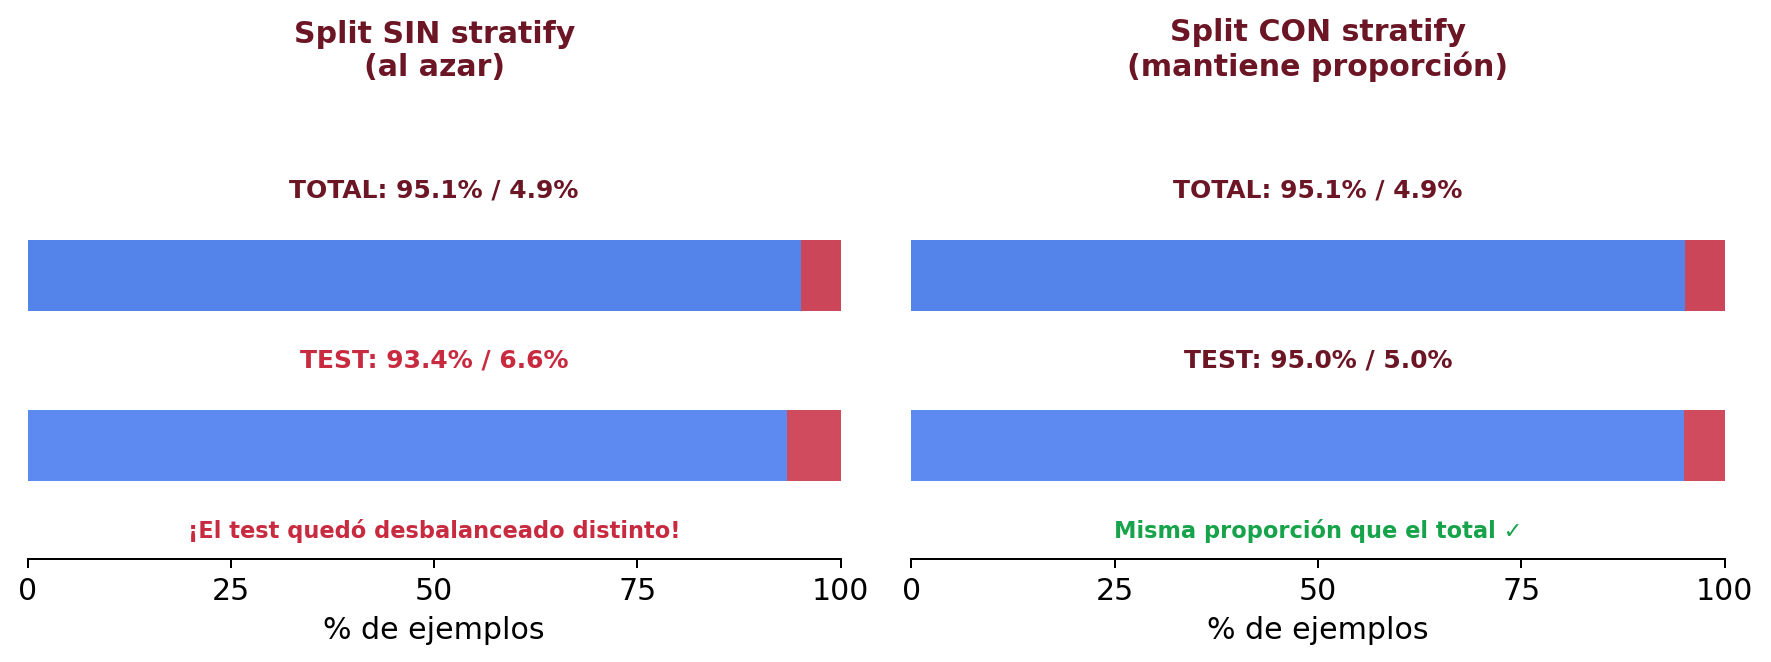
\includegraphics[width=0.88\textwidth]{fig_stratify.png}
  \end{center}

  \vspace{2pt}
  {\scriptsize\color{textMuted}
  \begin{itemize}\setlength{\itemsep}{3pt}
    \item[{\color{arcaRed}\scriptsize\faArrowRight}]
      \textbf{Sin stratify}: el test puede quedar con una proporción de
      positivos distinta a la del dataset original.
    \item[{\color{codeGreen}\scriptsize\faArrowRight}]
      \textbf{Con stratify}: la proporción se mantiene $\approx$ idéntica
      entre train, test y total.
  \end{itemize}
  }
\end{frame}

\begin{frame}[fragile,shrink=32]{Entrenar y Evaluar --- Honestamente}
  \vspace{-6pt}
  \begin{pyblock}
from sklearn.preprocessing import StandardScaler
from sklearn.linear_model import LogisticRegression
from sklearn.metrics import accuracy_score, recall_score, precision_score

# Escalar SOLO con train (evitar data leakage)
scaler = StandardScaler()
X_train_s = scaler.fit_transform(X_train)
X_test_s  = scaler.transform(X_test)   # solo transform, NO fit

modelo = LogisticRegression(max_iter=1000, class_weight="balanced")
modelo.fit(X_train_s, y_train)

y_pred_train = modelo.predict(X_train_s)
y_pred_test  = modelo.predict(X_test_s)

print(f"Accuracy train: {accuracy_score(y_train, y_pred_train):.3f}")
print(f"Accuracy test:  {accuracy_score(y_test,  y_pred_test):.3f}")
print(f"Recall test:    {recall_score(y_test,    y_pred_test):.3f}")
  \end{pyblock}

  \vspace{4pt}
  {\scriptsize\color{arcaRed}
    \faExclamationTriangle\hspace{4pt}\textbf{Data leakage}: el
    \texttt{scaler} se ajusta \textbf{solo con train}. Si usamos
    \texttt{fit\_transform} sobre todo el dataset, test ``ya vio'' información.}
\end{frame}

\begin{frame}[shrink=5]{Ejercicio 2: Tu Primer Split Honesto}
  \vspace{-4pt}
  {\footnotesize\color{arcaDark}\bfseries
    \faClock\hspace{4pt} 10 minutos --- Con el dataset de stroke:}

  \vspace{6pt}
  {\footnotesize
  \begin{enumerate}\setlength{\itemsep}{4pt}
    \item Prepara \texttt{X} e \texttt{y} (ya hecho arriba).
    \item Aplica \texttt{train\_test\_split} con \texttt{test\_size=0.2},
      \texttt{random\_state=42} y \texttt{stratify=y}.
    \item Verifica que la proporción de positivos sea similar en train y test.
    \item Escala con \texttt{StandardScaler} (solo fit con train).
    \item Entrena logística balanced y reporta accuracy, precision y recall
      \textbf{en test}.
    \item Compara: ¿las métricas en test son peores que en train?
      \textit{¿Cuánto peores?}
  \end{enumerate}
  }
\end{frame}

% =============================================================================
%  BLOQUE D: CURVA ROC
% =============================================================================
\sectionframe{Curva ROC y AUC}{Más allá del umbral 0.5}

\begin{frame}[shrink=22]{El Modelo No Devuelve Etiquetas, Devuelve Probabilidades}
  \vspace{-4pt}
  {\footnotesize\color{arcaDark}\bfseries
    Cuando la regresión logística ``predice'', realmente responde:
    \textit{``hay un 67\% de probabilidad de que este paciente sufra un ACV''}.}

  \vspace{6pt}
  \begin{center}
    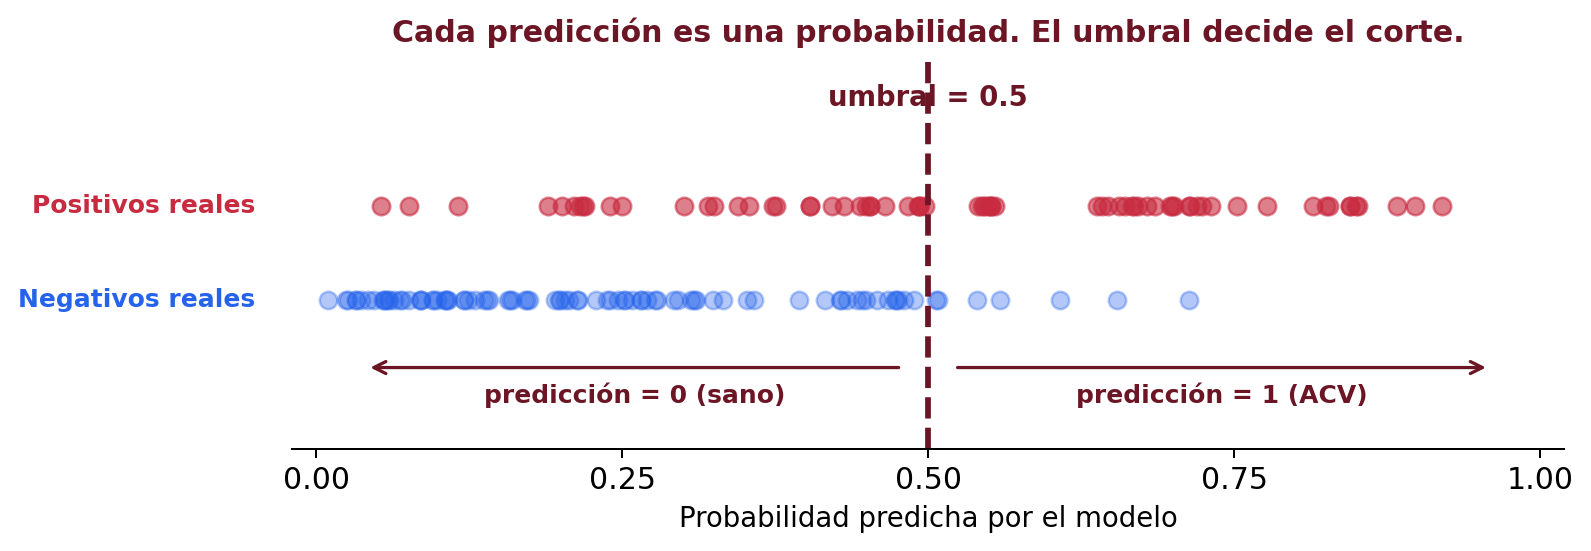
\includegraphics[width=0.85\textwidth]{fig_umbral.png}
  \end{center}

  \vspace{2pt}
  {\scriptsize\color{textMuted}
    Cada punto es un paciente. Rojo = tuvo ACV, azul = sano.
    La línea vertical es el \textbf{umbral}: todo lo que caiga a la derecha
    se clasifica como ``1'', a la izquierda como ``0''.}
\end{frame}

\begin{frame}[fragile,shrink=10]{\texttt{predict\_proba()} y el Umbral 0.5}
  \vspace{-4pt}
  {\footnotesize\color{arcaDark}\bfseries
    \texttt{predict()} usa por defecto un umbral de \textbf{0.5}.
    Pero 0.5 es una convención, no una ley.}

  \vspace{4pt}
  \begin{pyblock}
# Probabilidades reales del modelo
probs = modelo.predict_proba(X_test_s)[:, 1]
print(probs[:5])
# -> [0.08, 0.42, 0.67, 0.15, 0.91]

# Esto es lo que predict() hace internamente:
y_pred_default = (probs >= 0.5).astype(int)

# Pero podemos elegir OTRO umbral:
y_pred_sensible = (probs >= 0.3).astype(int)   # mas alertas
y_pred_estricto = (probs >= 0.7).astype(int)   # mas confianza
  \end{pyblock}

  \vspace{2pt}
  {\scriptsize\color{arcaDark}
    \faKey\hspace{4pt} El umbral es una \textbf{decisión de negocio}, no
    estadística. Lo elegimos según el costo del error.}
\end{frame}

\begin{frame}{La Curva ROC --- ¿Qué Mide?}
  \vspace{-4pt}
  {\footnotesize\color{arcaDark}\bfseries
    La curva \textbf{ROC} (Receiver Operating Characteristic) muestra cómo
    se comportan \texttt{TPR} y \texttt{FPR} para \textbf{cada umbral posible}.}

  \vspace{6pt}
  {\scriptsize
  \begin{tabular}{@{}lp{9cm}@{}}
    \toprule
    \textbf{TPR} (True Positive Rate) & \texttt{= VP / (VP + FN)} --- el \textbf{recall}. De los enfermos, ¿cuántos detecto? \\
    \textbf{FPR} (False Positive Rate) & \texttt{= FP / (FP + VN)} --- de los sanos, ¿a cuántos marqué mal como enfermos? \\
    \bottomrule
  \end{tabular}
  }

  \vspace{8pt}
  {\footnotesize
  \begin{itemize}\setlength{\itemsep}{4pt}
    \item[{\color{arcaRed}\scriptsize\faArrowRight}]
      \textbf{Umbral muy bajo} (0.01): detecto a todos (TPR=1) pero también
      marco sanos (FPR alto).
    \item[{\color{arcaRed}\scriptsize\faArrowRight}]
      \textbf{Umbral muy alto} (0.99): casi no marco a nadie (TPR=0, FPR=0).
    \item[{\color{arcaRed}\scriptsize\faArrowRight}]
      \textbf{La curva recorre todos esos puntos.}
  \end{itemize}
  }
\end{frame}

\begin{frame}{Cómo Se Calcula CADA Punto de la ROC}
  \vspace{-4pt}
  {\footnotesize\color{arcaDark}\bfseries
    Receta para \textbf{un} punto de la curva:}

  \vspace{4pt}
  {\footnotesize
  \begin{enumerate}\setlength{\itemsep}{3pt}
    \item Fijar un umbral $u$ (por ejemplo 0.20, 0.45, 0.70\ldots).
    \item Convertir probabilidades en predicciones: \texttt{y\_pred = (proba >= u)}.
    \item Contar VP, FN, FP, VN en la matriz de confusión.
    \item Calcular:
      $\text{TPR} = \dfrac{VP}{VP + FN}$, \quad
      $\text{FPR} = \dfrac{FP}{FP + VN}$
    \item Graficar el punto $(\text{FPR}, \text{TPR})$.
  \end{enumerate}
  }

  \vspace{4pt}
  \begin{tcolorbox}[colback=arcaRed!8, colframe=arcaRed, boxrule=0.5pt,
    arc=2pt, left=6pt, right=6pt, top=4pt, bottom=4pt]
    {\scriptsize\color{arcaDark}
    \faArrowRight\hspace{4pt}\textbf{Repetir} para \textbf{todos} los umbrales posibles
    (sklearn lo hace automáticamente, usando los scores únicos como umbrales).
    Los puntos conectados forman la curva.}
  \end{tcolorbox}
\end{frame}

\begin{frame}[shrink=42]{3 Umbrales = 3 Puntos en la Curva}
  \vspace{-4pt}
  \begin{center}
    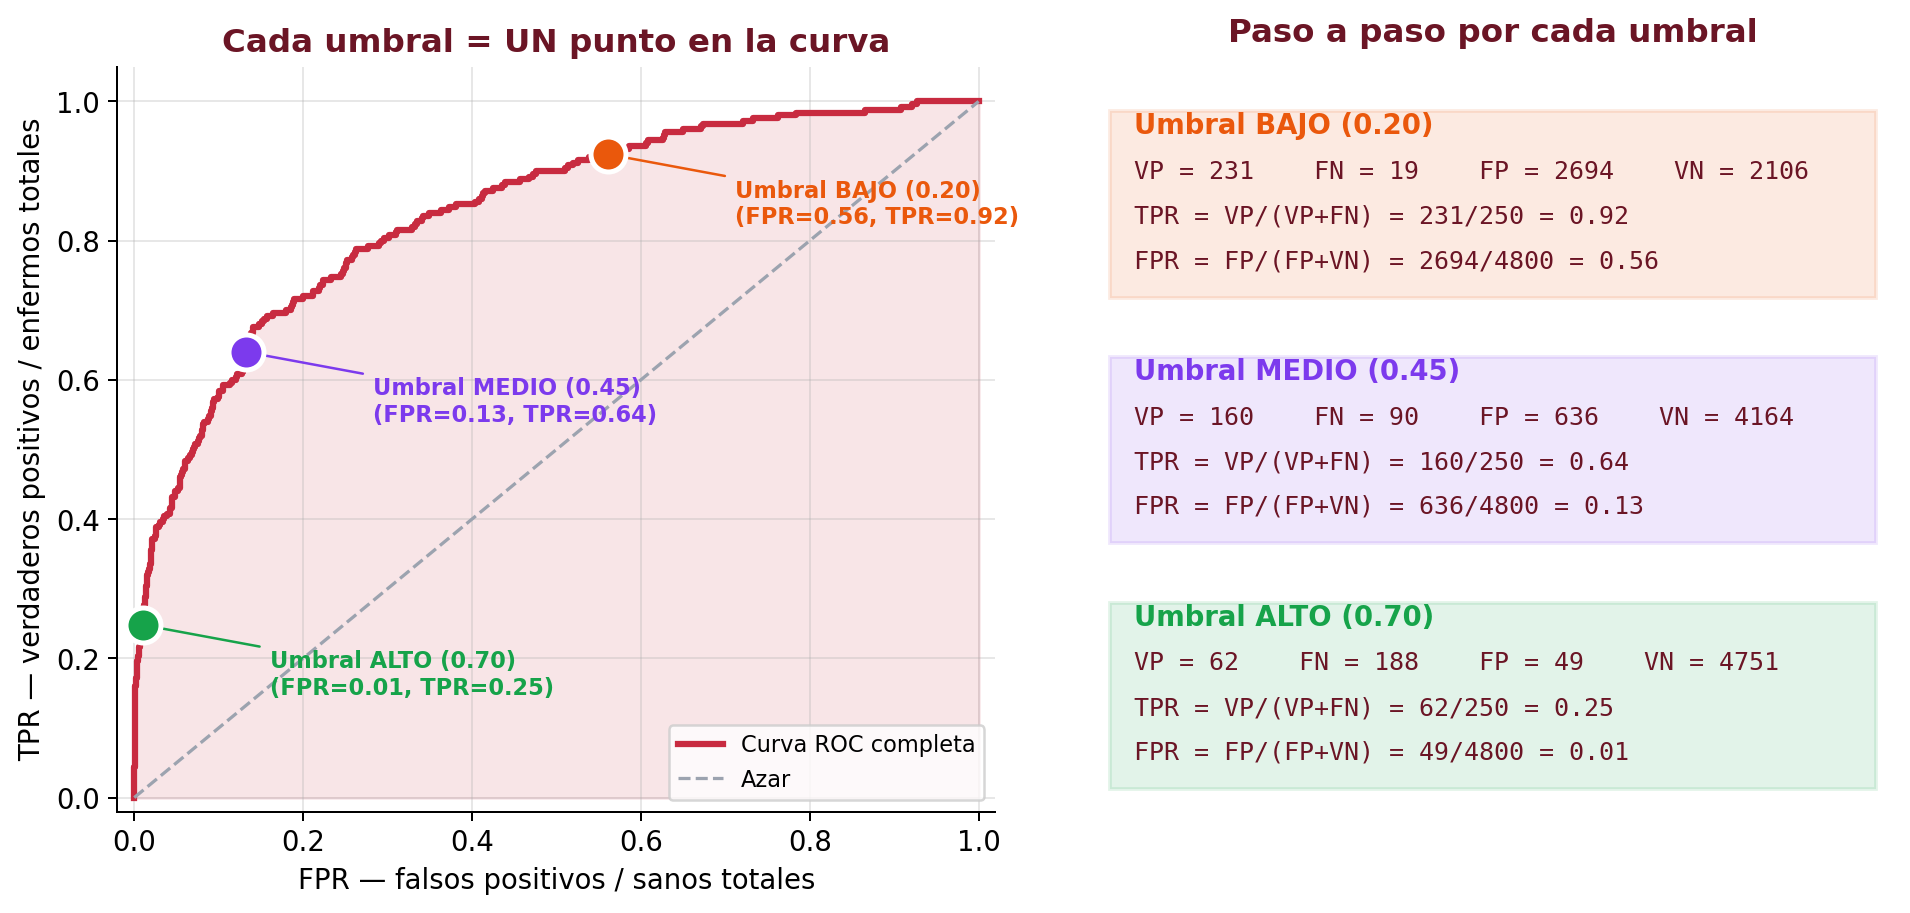
\includegraphics[width=0.82\textwidth]{fig_roc_puntos.png}
  \end{center}

  \vspace{-2pt}
  {\scriptsize\color{textMuted}
    \faLightbulb\hspace{4pt} Mismo modelo, mismos datos. Cambiando el
    umbral obtenemos puntos \textbf{distintos}. La curva es el lugar
    geométrico de TODOS los umbrales.}
\end{frame}

\begin{frame}[shrink=20]{¿Cómo Se Calcula el AUC?}
  \vspace{-4pt}
  {\footnotesize\color{arcaDark}\bfseries
    AUC = \textbf{Área Bajo la Curva}. No es ``sumar y dividir''
    --- es una integral numérica.}

  \vspace{6pt}
  \begin{columns}[T]
    \begin{column}{0.58\textwidth}
      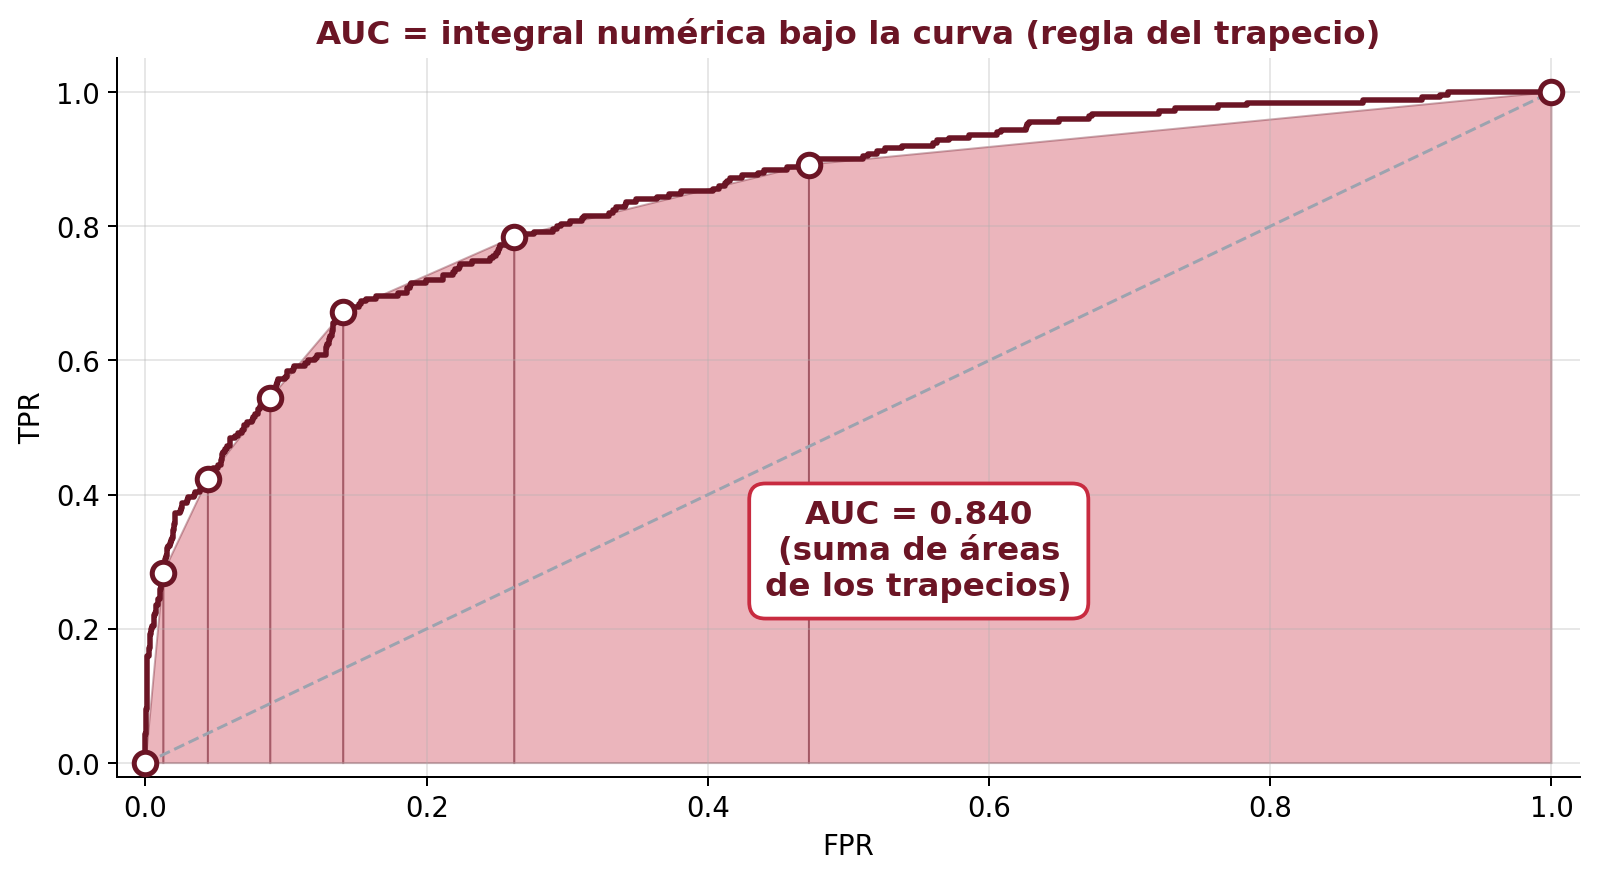
\includegraphics[width=\textwidth]{fig_auc_trapecios.png}
    \end{column}
    \begin{column}{0.40\textwidth}
      {\scriptsize\color{arcaDark}
      \textbf{Regla del trapecio:}
      \vspace{4pt}

      Entre dos puntos consecutivos $(x_i, y_i)$ y $(x_{i+1}, y_{i+1})$:
      $$\text{área}_i = (x_{i+1} - x_i) \cdot \frac{y_i + y_{i+1}}{2}$$

      \vspace{4pt}
      AUC total:
      $$\text{AUC} = \sum_i \text{área}_i$$

      \vspace{4pt}
      \texttt{sklearn.metrics.auc} hace exactamente esto.}
    \end{column}
  \end{columns}

  \vspace{4pt}
  {\scriptsize\color{textMuted}
    \faArrowRight\hspace{4pt} \textbf{Interpretación probabilística:} el AUC
    es la probabilidad de que el modelo dé un score más alto a un enfermo
    aleatorio que a un sano aleatorio. AUC = 0.84 → 84\% de las veces
    acierta el orden.}
\end{frame}

\begin{frame}[shrink=26]{Cómo Se Lee la Curva ROC}
  \vspace{-4pt}
  \begin{center}
    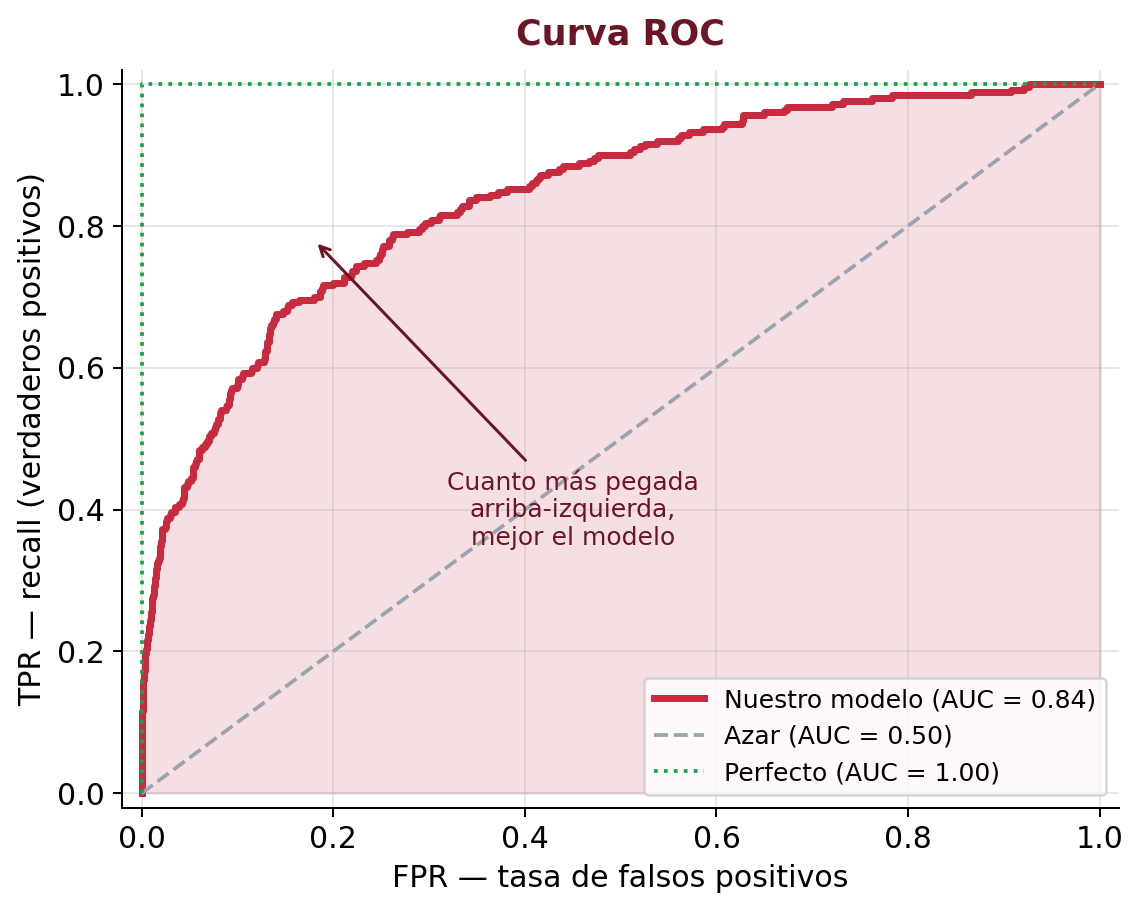
\includegraphics[width=0.5\textwidth]{fig_roc.png}
  \end{center}

  \vspace{-4pt}
  {\scriptsize\color{textMuted}
    \faLightbulb\hspace{4pt} \textbf{AUC} = área bajo la curva.
    1.0 = perfecto, 0.5 = azar, $\geq$ 0.8 se considera ``bueno''.
    Cuanto más arriba-izquierda esté la curva, mejor.}
\end{frame}

\begin{frame}[fragile,shrink=18]{Calcular y Graficar la Curva ROC}
  \vspace{-6pt}
  \begin{pyblock}
from sklearn.metrics import roc_curve, roc_auc_score
import plotly.express as px
import plotly.graph_objects as go

y_proba = modelo.predict_proba(X_test_s)[:, 1]
fpr, tpr, thresh = roc_curve(y_test, y_proba)
auc = roc_auc_score(y_test, y_proba)

fig = px.area(x=fpr, y=tpr,
    title=f"Curva ROC (AUC = {auc:.3f})",
    labels={"x": "FPR (1 - Especificidad)", "y": "TPR (Recall)"})
fig.add_shape(type="line", line=dict(dash="dash"),
              x0=0, x1=1, y0=0, y1=1)
fig.show()
  \end{pyblock}

  \vspace{4pt}
  {\scriptsize\color{textMuted}
    \faMousePointer\hspace{4pt} Con Plotly, al pasar el mouse se ven
    los valores exactos de cada punto (FPR, TPR).}
\end{frame}

% =============================================================================
%  BLOQUE E: CURVA PR
% =============================================================================
\sectionframe{Curva Precision-Recall}{La correcta para desbalanceados}

\begin{frame}{¿Por Qué PR > ROC en Datos Desbalanceados?}
  \vspace{-4pt}
  {\footnotesize\color{arcaDark}\bfseries
    La curva ROC puede verse ``bonita'' incluso cuando el modelo es malo
    --- si el desbalance es fuerte.}

  \vspace{6pt}
  {\footnotesize
  \begin{itemize}\setlength{\itemsep}{4pt}
    \item[{\color{arcaRed}\scriptsize\faArrowRight}]
      El FPR tiene un denominador \textbf{enorme} (todos los sanos).
      Unos pocos falsos positivos ``se diluyen''.
    \item[{\color{arcaRed}\scriptsize\faArrowRight}]
      Ejemplo: 100 falsos positivos sobre 4861 sanos →
      FPR = 2\%. \textit{Parece bueno.}
    \item[{\color{arcaRed}\scriptsize\faArrowRight}]
      Pero si solo hay 249 positivos reales y detectamos 50,
      la \textbf{precisión} es 50/(50+100) = 33\%. \textit{Es malo.}
  \end{itemize}
  }

  \vspace{6pt}
  \begin{tcolorbox}[colback=arcaRed!8, colframe=arcaRed, boxrule=0.5pt,
    arc=2pt, left=6pt, right=6pt, top=4pt, bottom=4pt]
    {\scriptsize\color{arcaDark}
    \faKey\hspace{4pt}\textbf{Regla:} datos muy desbalanceados → usen
    \textbf{Precision-Recall}, no ROC. La PR se centra solo en la
    clase positiva (la que nos importa).}
  \end{tcolorbox}
\end{frame}

\begin{frame}[shrink=35]{Curva PR --- Los Ejes}
  \vspace{-4pt}
  \begin{center}
    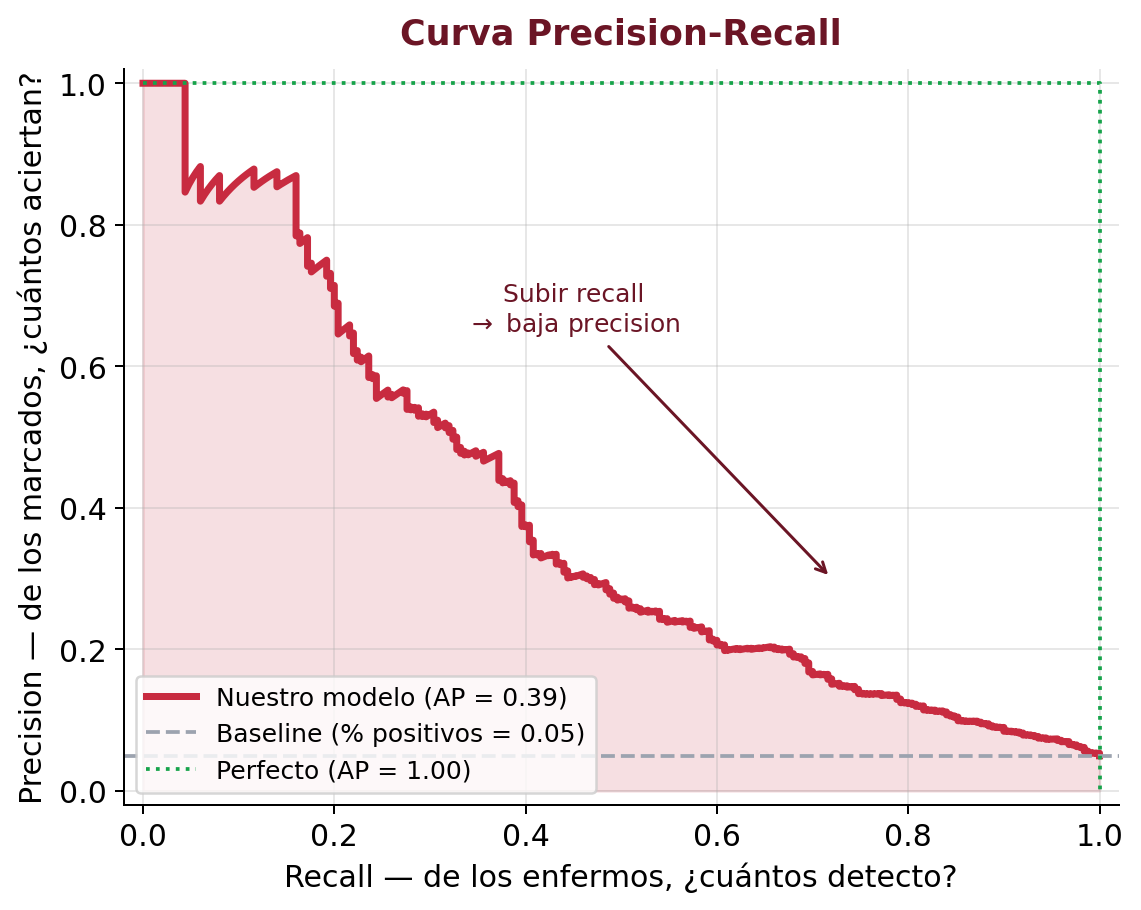
\includegraphics[width=0.5\textwidth]{fig_pr.png}
  \end{center}

  \vspace{-4pt}
  {\scriptsize\color{textMuted}
    \faLightbulb\hspace{4pt}
    \textbf{Precision} = VP / (VP + FP): de los que marqué, ¿cuántos son reales?
    \quad\textbf{Recall} = VP / (VP + FN): de los reales, ¿cuántos marqué?
    \quad\textbf{Trade-off}: subir uno baja el otro.}
\end{frame}

\begin{frame}{Cómo Se Calcula CADA Punto de la PR}
  \vspace{-4pt}
  {\footnotesize\color{arcaDark}\bfseries
    Misma receta que ROC, \textbf{cambia solo el eje}:}

  \vspace{4pt}
  {\footnotesize
  \begin{enumerate}\setlength{\itemsep}{3pt}
    \item Fijar un umbral $u$.
    \item \texttt{y\_pred = (proba >= u)}.
    \item Contar VP, FN, FP, VN.
    \item Calcular:
      $\text{Precision} = \dfrac{VP}{VP + FP}$, \quad
      $\text{Recall} = \dfrac{VP}{VP + FN}$
    \item Graficar el punto $(\text{Recall}, \text{Precision})$.
  \end{enumerate}
  }

  \vspace{4pt}
  \begin{tcolorbox}[colback=arcaRed!8, colframe=arcaRed, boxrule=0.5pt,
    arc=2pt, left=6pt, right=6pt, top=4pt, bottom=4pt]
    {\scriptsize\color{arcaDark}
    \faKey\hspace{4pt}\textbf{Diferencia con ROC:} el eje X ahora es el mismo
    (Recall = TPR), pero el Y es \textbf{Precision} (no FPR). La precisión
    \textit{ignora los verdaderos negativos} → se concentra en la clase positiva.}
  \end{tcolorbox}
\end{frame}

\begin{frame}[shrink=42]{3 Umbrales = 3 Puntos en la Curva PR}
  \vspace{-4pt}
  \begin{center}
    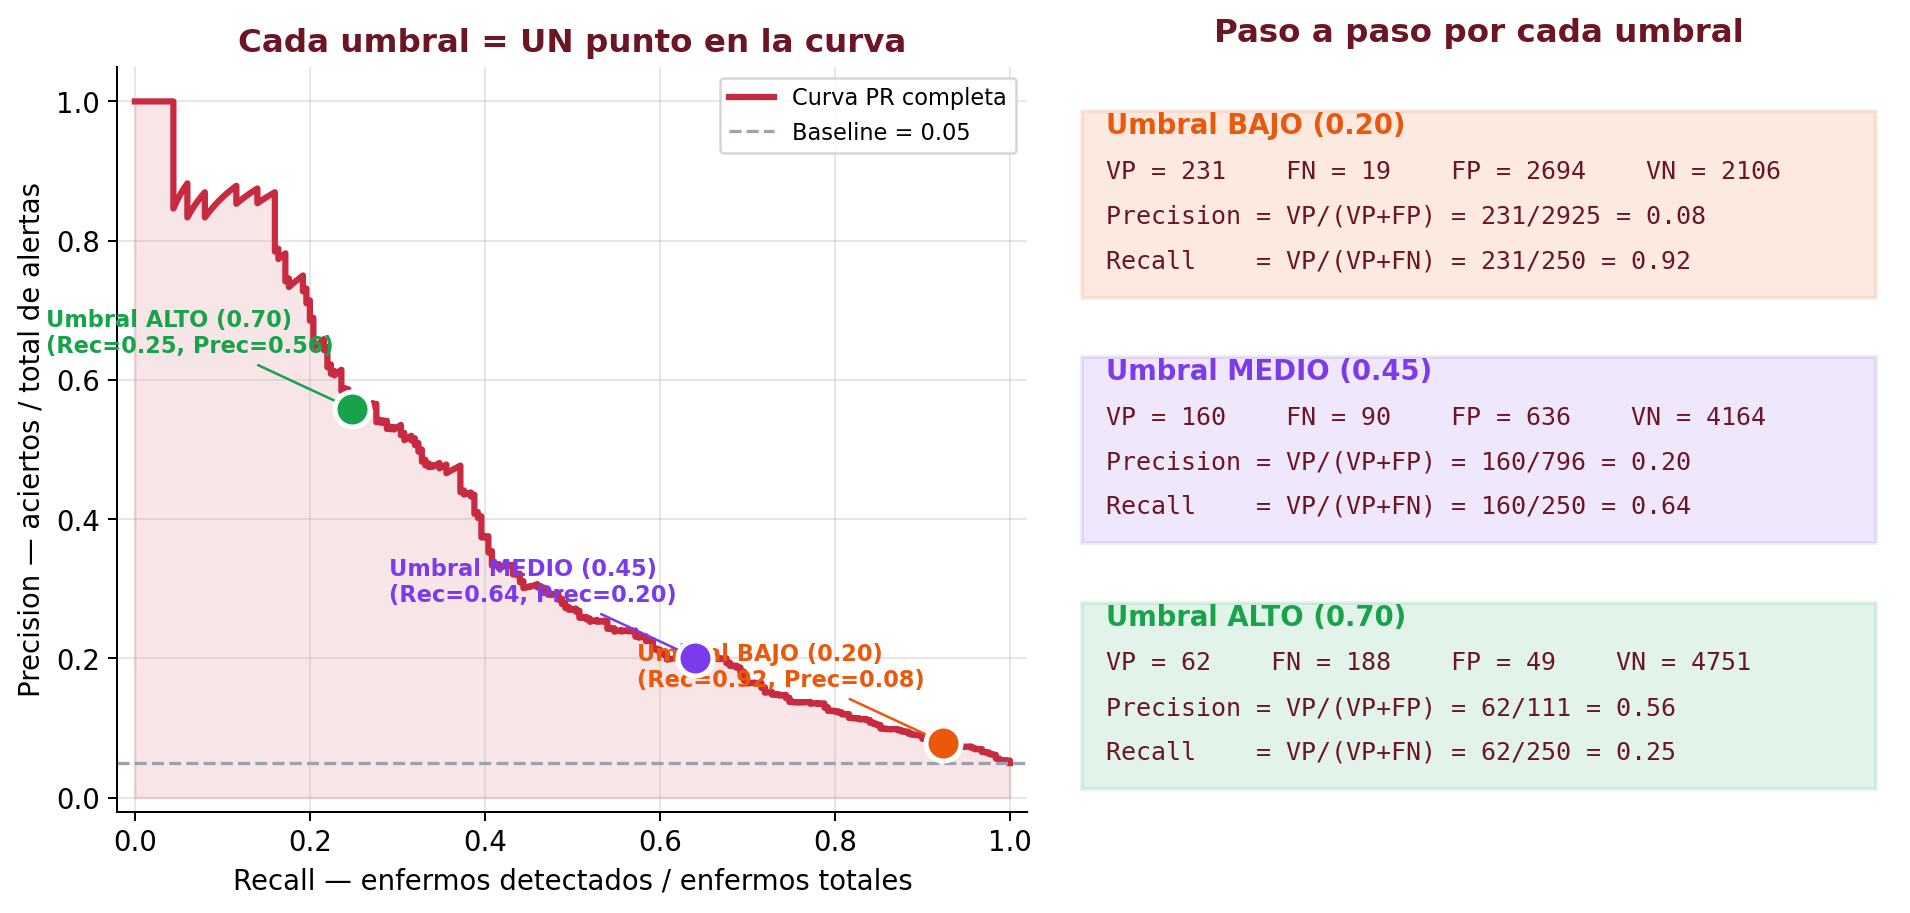
\includegraphics[width=0.82\textwidth]{fig_pr_puntos.png}
  \end{center}

  \vspace{-2pt}
  {\scriptsize\color{textMuted}
    \faLightbulb\hspace{4pt} Con \textbf{umbral alto} (verde) la precisión
    sube pero el recall cae → detectamos pocos pero acertamos. Con
    \textbf{umbral bajo} (naranja) es al revés.}
\end{frame}

\begin{frame}[shrink=15]{¿Cómo Se Calcula el AP (Average Precision)?}
  \vspace{-4pt}
  {\footnotesize\color{arcaDark}\bfseries
    AP = área bajo la curva PR. Pero sklearn lo calcula \textbf{distinto} al AUC.}

  \vspace{6pt}
  {\footnotesize
  \begin{itemize}\setlength{\itemsep}{4pt}
    \item[{\color{arcaRed}\scriptsize\faArrowRight}]
      \textbf{Promedio ponderado} de la precisión en cada punto, pesado por
      cuánto subió el recall:
      $$\text{AP} = \sum_n (R_n - R_{n-1}) \cdot P_n$$
    \item[{\color{arcaRed}\scriptsize\faArrowRight}]
      Es una \textbf{suma de rectángulos} (no trapecios como AUC) --- esto
      evita sobrestimar la curva, que es ``escalonada'' en PR.
    \item[{\color{arcaRed}\scriptsize\faArrowRight}]
      Un modelo \textbf{aleatorio} tiene AP = proporción de positivos
      (en stroke, AP aleatorio $\approx$ 0.05).
  \end{itemize}
  }

  \vspace{4pt}
  \begin{tcolorbox}[colback=codeGreen!8, colframe=codeGreen, boxrule=0.5pt,
    arc=2pt, left=6pt, right=6pt, top=4pt, bottom=4pt]
    {\scriptsize\color{arcaDark}
    \faLightbulb\hspace{4pt} Lee: un AP de 0.30 en datos con 5\% de positivos
    significa que el modelo es \textbf{6x mejor que el azar} al rankear
    los positivos arriba.}
  \end{tcolorbox}
\end{frame}

\begin{frame}[fragile,shrink=18]{Calcular y Graficar la Curva PR}
  \vspace{-6pt}
  \begin{pyblock}
from sklearn.metrics import precision_recall_curve, average_precision_score

prec, rec, thr = precision_recall_curve(y_test, y_proba)
ap = average_precision_score(y_test, y_proba)

fig = px.area(x=rec, y=prec,
    title=f"Curva Precision-Recall (AP = {ap:.3f})",
    labels={"x": "Recall", "y": "Precision"})

# Linea de baseline (prevalencia)
fig.add_hline(y=y_test.mean(), line_dash="dash",
              annotation_text="baseline (% positivos)")
fig.show()
  \end{pyblock}

  \vspace{4pt}
  {\scriptsize\color{textMuted}
  \begin{itemize}\setlength{\itemsep}{3pt}
    \item[{\color{arcaRed}\scriptsize\faArrowRight}]
      \textbf{AP} (Average Precision): área bajo la curva PR.
      En datos muy desbalanceados, un AP de 0.30 ya es \textit{notable}
      (baseline es 0.05).
  \end{itemize}
  }
\end{frame}

% =============================================================================
%  BLOQUE F: UMBRAL
% =============================================================================
\sectionframe{Umbral Óptimo}{Llevando la evaluación al negocio}

\begin{frame}{El Costo del Error NO Es Simétrico}
  \vspace{-4pt}
  {\footnotesize\color{arcaDark}\bfseries
    En un hospital:}

  \vspace{6pt}
  \begin{columns}[T]
    \begin{column}{0.48\textwidth}
      \begin{tcolorbox}[colback=arcaRed!10, colframe=arcaRed, boxrule=0.5pt,
        arc=2pt, title={\small\color{white}\bfseries\faHeartbeat\ Falso Negativo}]
        {\scriptsize
        Paciente \textbf{tiene} riesgo, el modelo dice que no.
        \vspace{3pt}
        \begin{itemize}\setlength{\itemsep}{2pt}
          \item Costo: \textbf{vida humana}
          \item Valor: \$\$\$\$\$
        \end{itemize}
        }
      \end{tcolorbox}
    \end{column}
    \begin{column}{0.48\textwidth}
      \begin{tcolorbox}[colback=codeOrange!10, colframe=codeOrange, boxrule=0.5pt,
        arc=2pt, title={\small\color{white}\bfseries\faStethoscope\ Falso Positivo}]
        {\scriptsize
        Paciente \textbf{no tiene} riesgo, el modelo dice que sí.
        \vspace{3pt}
        \begin{itemize}\setlength{\itemsep}{2pt}
          \item Costo: chequeo adicional
          \item Valor: \$
        \end{itemize}
        }
      \end{tcolorbox}
    \end{column}
  \end{columns}

  \vspace{8pt}
  {\footnotesize\color{arcaDark}
    \faArrowRight\hspace{4pt} En medicina, preferimos \textbf{recall alto}
    aunque la precisión baje. Esto implica \textbf{bajar el umbral}
    por debajo de 0.5.}
\end{frame}

\begin{frame}[fragile,shrink=28]{Explorar Umbrales}
  \vspace{-6pt}
  \begin{pyblock}
import numpy as np
import pandas as pd

umbrales = np.arange(0.1, 0.9, 0.05)
resultados = []
for u in umbrales:
    y_pred_u = (y_proba >= u).astype(int)
    resultados.append({
        "umbral": u,
        "precision": precision_score(y_test, y_pred_u, zero_division=0),
        "recall":    recall_score(y_test, y_pred_u),
    })
df_u = pd.DataFrame(resultados)

fig = px.line(df_u.melt(id_vars="umbral"),
              x="umbral", y="value", color="variable",
              title="Precision y Recall vs Umbral")
fig.show()
  \end{pyblock}
\end{frame}

\begin{frame}{Elegir el Umbral con Lógica de Negocio}
  \vspace{-4pt}
  {\footnotesize\color{arcaDark}\bfseries
    Tres estrategias comunes:}

  \vspace{6pt}
  {\footnotesize
  \begin{enumerate}\setlength{\itemsep}{6pt}
    \item[{\color{arcaRed}\bfseries 1.}]
      \textbf{F1 máximo}: balance precision-recall.\\
      \texttt{f1 = 2 * P * R / (P + R)} --- útil cuando no hay preferencia clara.
    \item[{\color{arcaRed}\bfseries 2.}]
      \textbf{Recall mínimo}: ``detecta al menos 80\% de los ACV''.
      Buscar el umbral más alto que cumpla → menos falsos positivos posibles.
    \item[{\color{arcaRed}\bfseries 3.}]
      \textbf{Costo esperado}: multiplicar errores por su costo y minimizar.\\
      \texttt{costo = FN * c\_FN + FP * c\_FP}
  \end{enumerate}
  }

  \vspace{6pt}
  \begin{tcolorbox}[colback=arcaGray, colframe=arcaRed, boxrule=0.5pt, arc=2pt,
    left=6pt, right=6pt, top=4pt, bottom=4pt]
    {\scriptsize\color{arcaDark}
    \faLightbulb\hspace{4pt} Si un FN cuesta \$10.000 (tratamiento tardío)
    y un FP cuesta \$200 (un chequeo), la razón es 50:1. El umbral
    óptimo será \textbf{mucho más bajo} que 0.5.}
  \end{tcolorbox}
\end{frame}

\begin{frame}[fragile,shrink=25]{Caso de Negocio: Umbral por Costo}
  \vspace{-6pt}
  \begin{pyblock}
COSTO_FN = 10_000   # no detectar ACV
COSTO_FP = 200      # falsa alarma

from sklearn.metrics import confusion_matrix
costos = []
for u in umbrales:
    y_pred_u = (y_proba >= u).astype(int)
    tn, fp, fn, tp = confusion_matrix(y_test, y_pred_u).ravel()
    costos.append({"umbral": u,
                   "costo": fn*COSTO_FN + fp*COSTO_FP})

df_c = pd.DataFrame(costos)
u_opt = df_c.loc[df_c["costo"].idxmin(), "umbral"]
print(f"Umbral optimo: {u_opt:.2f}")

px.line(df_c, x="umbral", y="costo",
        title=f"Costo esperado (optimo: {u_opt:.2f})").show()
  \end{pyblock}
\end{frame}

\begin{frame}[shrink=5]{Ejercicio 3: Tu Curva ROC y PR}
  \vspace{-4pt}
  {\footnotesize\color{arcaDark}\bfseries
    \faClock\hspace{4pt} 12 minutos --- con el modelo que entrenaron arriba:}

  \vspace{6pt}
  {\footnotesize
  \begin{enumerate}\setlength{\itemsep}{4pt}
    \item Obtengan \texttt{y\_proba = modelo.predict\_proba(X\_test\_s)[:, 1]}.
    \item Calculen y grafiquen la \textbf{curva ROC} con Plotly. Reporten AUC.
    \item Calculen y grafiquen la \textbf{curva PR}. Reporten AP.
    \item Prueben 5 umbrales distintos (0.1, 0.3, 0.5, 0.7, 0.9).
      Para cada uno, reporten precision, recall y matriz de confusión.
    \item ¿Qué umbral eligirían si un FN cuesta 50x más que un FP?
  \end{enumerate}
  }
\end{frame}

\begin{frame}[shrink=5]{Ejercicio 4 (Retador): Comparar Modelos}
  \vspace{-4pt}
  {\footnotesize\color{arcaDark}\bfseries
    \faClock\hspace{4pt} 10 minutos:}

  \vspace{6pt}
  {\footnotesize
  \begin{enumerate}\setlength{\itemsep}{4pt}
    \item Entrenen \textbf{dos} modelos sobre el mismo train:
      \begin{itemize}\setlength{\itemsep}{2pt}
        \item Logística sin balancear (\texttt{class\_weight=None}).
        \item Logística con \texttt{class\_weight="balanced"}.
      \end{itemize}
    \item Grafiquen ambas curvas ROC \textbf{en el mismo gráfico}
      (\texttt{fig.add\_trace(...)}).
    \item ¿Cuál tiene mejor AUC? ¿Y mejor AP?
    \item Conclusión: ¿el desbalance afecta más al AUC o al AP?
  \end{enumerate}
  }
\end{frame}

% =============================================================================
%  CIERRE
% =============================================================================
\sectionframe{Cierre}{Lo que aprendimos hoy}

\begin{frame}[shrink=8]{Resumen}
  \vspace{-4pt}
  \begin{columns}[T]
    \begin{column}{0.48\textwidth}
      {\footnotesize\bfseries\color{arcaDark} Visualización:}
      \vspace{4pt}

      {\footnotesize
      \begin{itemize}\setlength{\itemsep}{4pt}
        \item[{\color{codeGreen}\faCheckCircle}]
          Plotly = interactivo (hover, zoom).
        \item[{\color{codeGreen}\faCheckCircle}]
          Matplotlib bajo nivel, Seaborn estadístico,
          Plotly dashboards.
        \item[{\color{codeGreen}\faCheckCircle}]
          \texttt{px.scatter/histogram/box/line}.
      \end{itemize}
      }
    \end{column}

    \begin{column}{0.48\textwidth}
      {\footnotesize\bfseries\color{arcaRed} Evaluación:}
      \vspace{4pt}

      {\footnotesize
      \begin{itemize}\setlength{\itemsep}{4pt}
        \item[{\color{codeGreen}\faCheckCircle}]
          \texttt{train\_test\_split} + \texttt{stratify}.
        \item[{\color{codeGreen}\faCheckCircle}]
          Curva ROC + AUC.
        \item[{\color{codeGreen}\faCheckCircle}]
          Curva PR + AP (la correcta para desbalance).
        \item[{\color{codeGreen}\faCheckCircle}]
          Umbral óptimo por costo de negocio.
      \end{itemize}
      }
    \end{column}
  \end{columns}

  \vspace{8pt}
  \begin{tcolorbox}[colback=arcaRed!8, colframe=arcaRed, boxrule=0.5pt, arc=2pt,
    left=6pt, right=6pt, top=4pt, bottom=4pt]
    {\scriptsize\color{arcaDark}
    \faArrowRight\hspace{4pt}\textbf{Próxima clase:} árboles de decisión
    --- un nuevo modelo, reutilizando todo este instrumental de evaluación.}
  \end{tcolorbox}
\end{frame}

% ── QR ENCUESTA ──────────────────────────────────────────────────────────────
{
\setbeamertemplate{headline}{}
\setbeamertemplate{footline}{}
\begin{frame}[plain, noframenumbering]
  \begin{tikzpicture}[remember picture, overlay]
    \fill[arcaDark] (current page.south west) rectangle (current page.north east);
  \end{tikzpicture}
  \vspace{1cm}
  \begin{center}
    {\Huge\bfseries\color{white} ¿Cómo estuvo la clase?\par}
    \vspace{0.6cm}
    
\includegraphics[width=4cm]{qr_encuesta.jpg}
    \vspace{0.4cm}

    {\large\color{white!80} Escanea el QR para dejarnos tu opinión.\par}
  \end{center}
\end{frame}
}

\end{document}
